\section*{\centering{Answers to the final questions sent on October 10th, 
2016}}


"Dear Mohammad,

After consultation of Raphael (who contacted you), the CAN review committee 
would like to request that the study of varying cut in the missing energy 
eHe4gX be repeated with a proper, bin dependent, pi0 subtraction. We understand 
that this may take several days, but feel it is a necessary step to raise any 
doubt about the stability of the result. Optionally, if time allows, add a 
fourth cut which would only get rid of the tails: [-0.45, 0.50].

I also discussed with Raphael the necessity to explain in the section on 
Systematic uncertainties how the corresponding numbers in the numerical tables 
are generated. So far, the discussion is exclusively on the fitted ALU(90$^\circ$), 
while the numbers in the Tables are bin-dependent.

Thank you and best regards,

Michel."

\begin{enumerate}
   \item \textcolor{blue}{Regarding the stability of the coherent $A_{LU}$ with 
      respect to the missing energy cut. We first remind the previous 
      exchange from the first round comments and the results we got. Then, we 
      present the new study after the CAN review committee suggestion.}
   
\begin{enumerate}
   \item The first round comment, where the background subtraction have been 
      performed based on the 4D background subtractions without binning in the 
      missing energy distribution: \\
      " 40) Fig.  4.2: I'm bothered by the wide distribution in Emiss (top 
      middle), and don't understand why you use such wide cuts.  Surely, 
      anything above Emiss = 0.4 must have additional particles in it, and even 
      if not, why not cut this tail?  Note that the same tail is absent for the 
      p (Fig. 4.6) where you use indeed a tighter cut, although you don't even 
      account for the proton's initial momentum.\\
   \textcolor{blue}{ We applied 3$\sigma$ based on the comparison between data 
      and simulation, see figure 4.4 in the note. In the following, figure 
      \ref{fig:coherent_ME_bins}, we performed bins in the missing energy 
      distribution and we watch the reconstructed beam-spin asymmetries. As a 
      conclusion, we see that the reconstructed asymmetries are compatible 
   within the given error bars.}" \\

\begin{figure}[tbp]
   \centering
   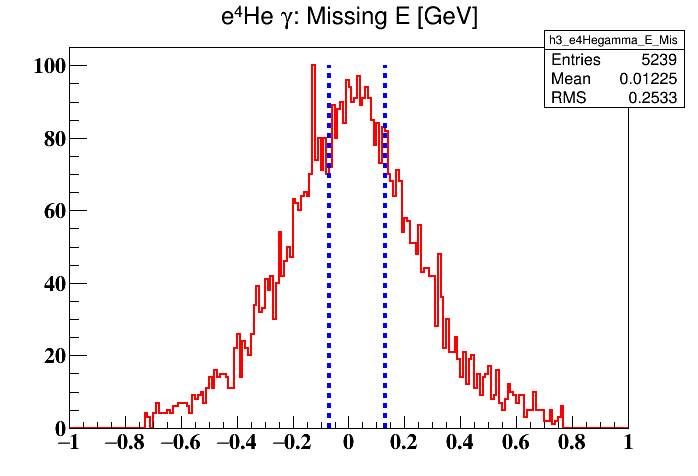
\includegraphics[height=7.0cm]{fig/coh_ME_bins.png}
   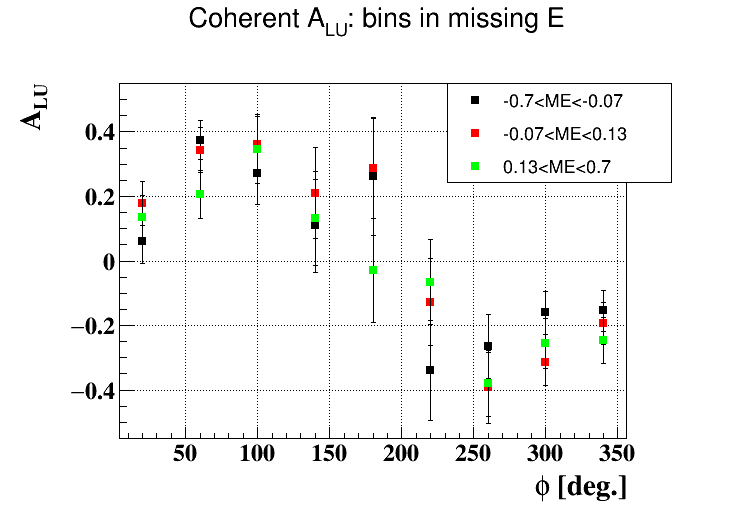
\includegraphics[height=7.0cm]{fig/BSA_coherent_ME.png}
   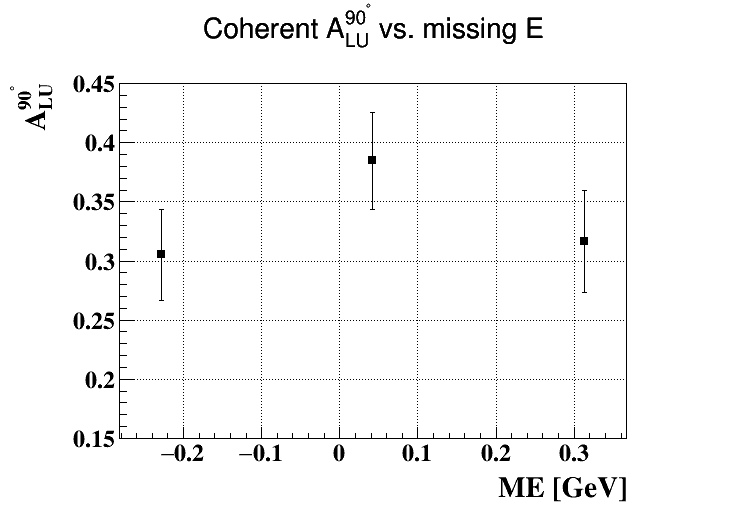
\includegraphics[height=7.0cm]{fig/coh_ME_alpha.png}
   \caption{Coherent missing energy distributions (top), the reconstructed 
   beam-spin asymmetries as a function of $\phi$ (middle), and the extracted 
asymmetry at $\phi = 90 ^{\circ}$ from fitting the asymmetries as a function of 
the missing energy in each bin. }
   \label{fig:coherent_ME_bins}
    \end{figure}


 \item Following the CAN committee suggestion, we performed this study again
    recalculating the $\pi^0$ contamination for the different bins in the 
    missing energy. The results are presented in figure 
    \ref{fig:coherent_ME_bins_2}. The high missing energy bin is the
    most affected and goes up, closer to the value from the central point.    
    This is easily understood as this bin has a significantly higher $\pi^0$
    contribution. In conclusion, the central bin remains with a stronger 
    signal, however we want to point out that (i) this feature is not significant 
    due to the large error bars in regard to the size of the effect and 
    (ii) the variations are smaller than the 8\% systematic error we evaluated 
    from the rather arbitrary choice of exclusivity cuts. In conclusion, we
    believe that the cut is good as it is. The main reason being that 
    statistical errors already dominate the error budget, so we think it
    would be counter productive to reduce even more our data sample in hope to
    reduce the systematic error.
   
    \begin{figure}[tbp]
     \centering
       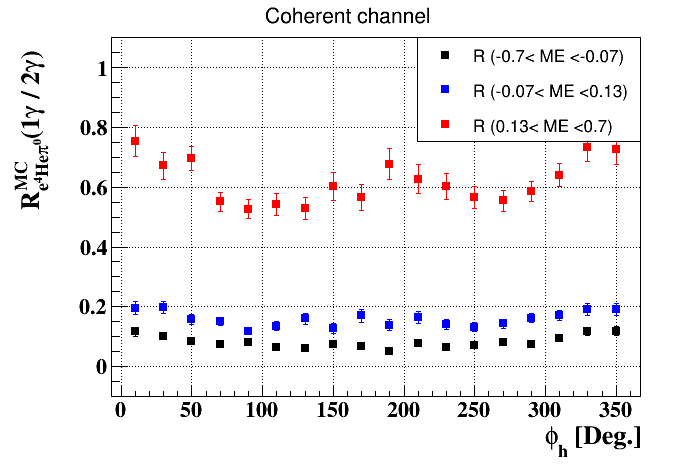
\includegraphics[height=6.5cm]{fig_new/e4Hegamma_e4Hepi0_Phi_ME.png}
       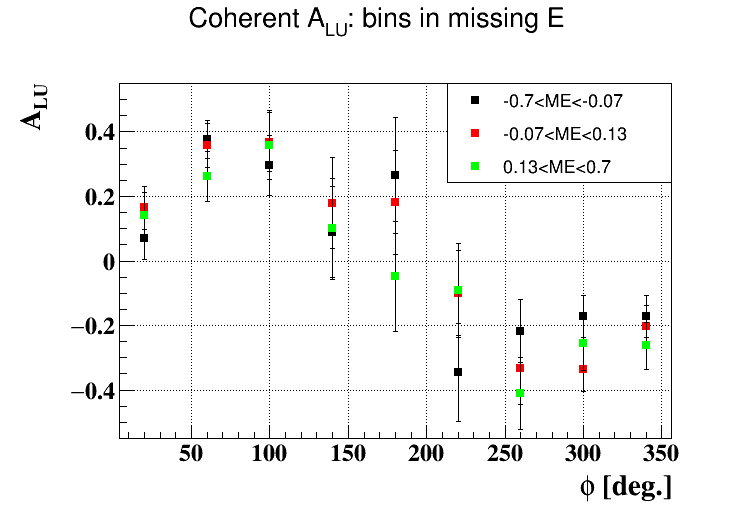
\includegraphics[height=6.5cm]{fig_new/BSA_coherent_ME.png}
       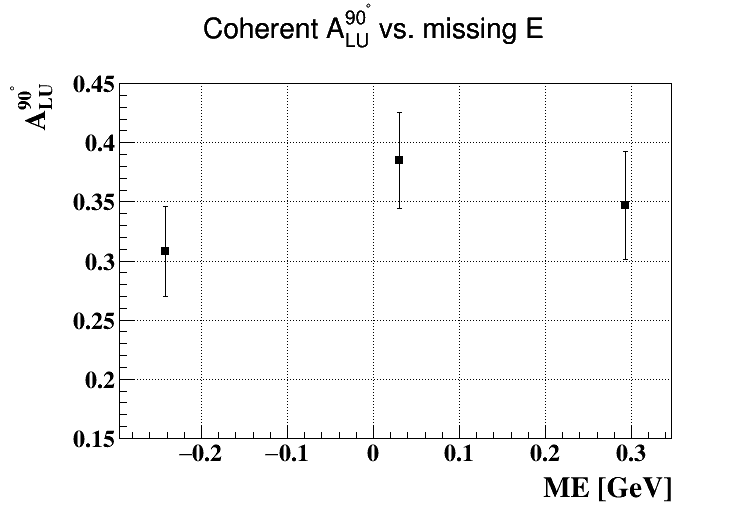
\includegraphics[height=6.5cm]{fig_new/coh_ME_alpha.png}
   \caption{From top to bottom, the corresponding background acceptance ratio 
in the different missing energy bins, the reconstructed beam-spin asymmetries 
as a function of $\phi$ (middle), and the extracted asymmetry at $\phi = 90 
^{\circ}$ from fitting the asymmetries as a function of the mean missing energy 
in each bin.}
   \label{fig:coherent_ME_bins_2}
    \end{figure}

 \item Regarding the request of cutting the tails and comparing the 
reconstructed coherent asymmetries to the ones without cutting the tails, the 
asymmetries are presented in fig \ref{fig:BSA_ME_bins_sig} as a function of 
$\phi$ in bins in $Q^{2}$, $x_{B}$ and $-t$. The $Q^{2}$, $x_{B}$ and $-t$ 
dependences of $A_{LU}$ at $\phi = 90 ^{\circ}$, from fitting the signals in 
fig \ref{fig:BSA_ME_bins_sig}, are presented in fig \ref{ig:ALU_ME_bins_sig} 
with and without cutting the tails in the missing energy distribution.  One can 
conclude that the two sets are compatible within the given error bars. 
   
    \begin{figure}[tbp]
     \centering
       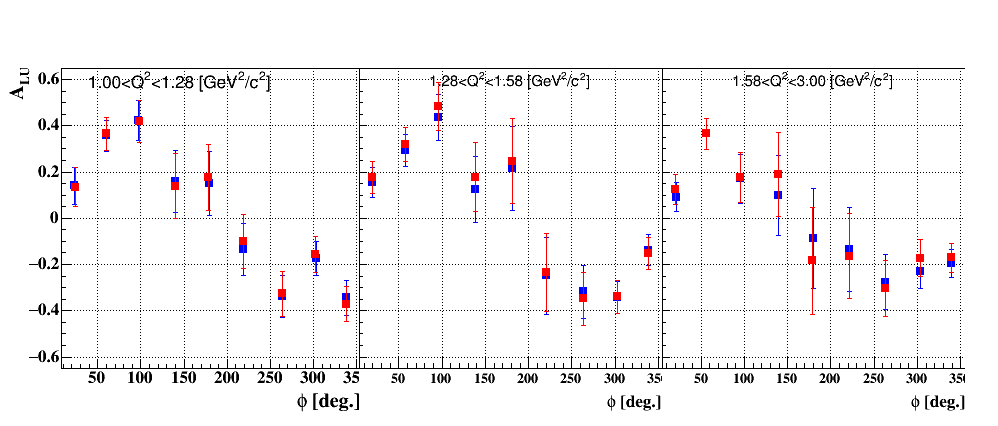
\includegraphics[height=6.5cm]{fig_new/BSA_Coh_Comb_Q2_ME.png}
       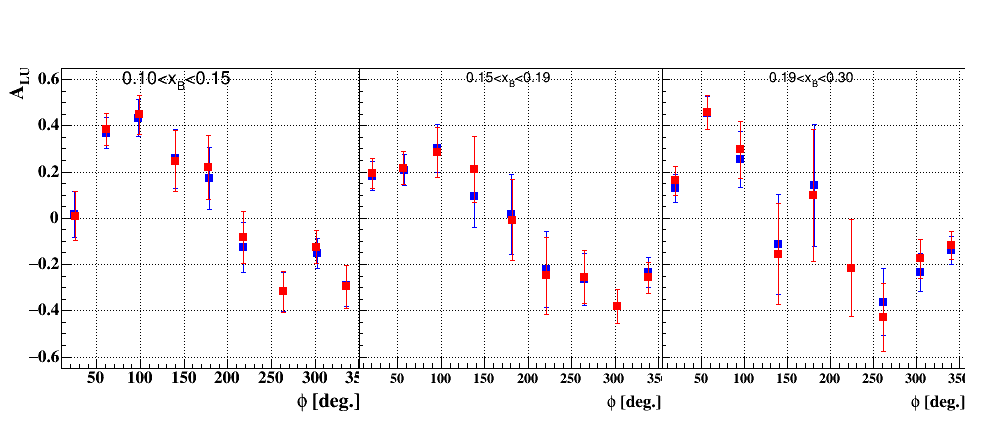
\includegraphics[height=6.5cm]{fig_new/BSA_Coh_Comb_xB_ME.png}
       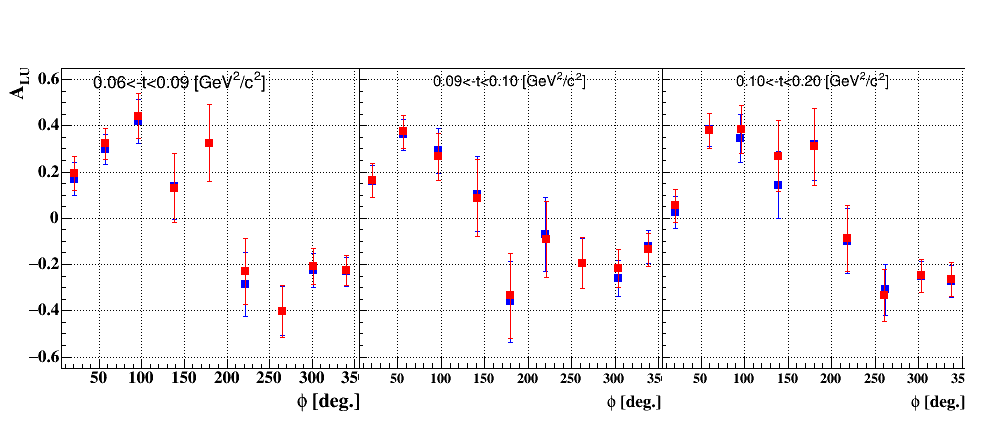
\includegraphics[height=6.5cm]{fig_new/BSA_Coh_Comb_t_ME.png}
   \caption{From top to bottom, the reconstructed beam-spin asymmetries as a 
      function of $\phi = 90 ^{\circ}$ in $Q^{2}$,
$x_{B}$ and $-t$ with cutting the tails in red and without cutting the tails in 
blue.  }
   \label{fig:BSA_ME_bins_sig}
    \end{figure}

    \begin{figure}[tbp]
     \centering
       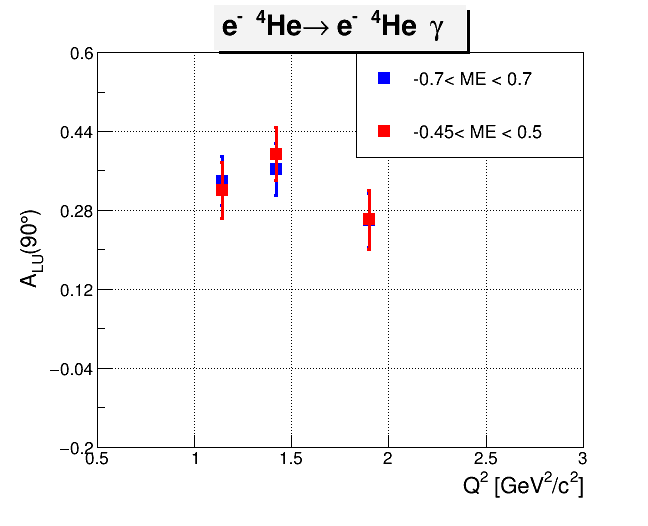
\includegraphics[height=7.5cm]{fig_new/A_LU_He_90_vs_Q2.png}
       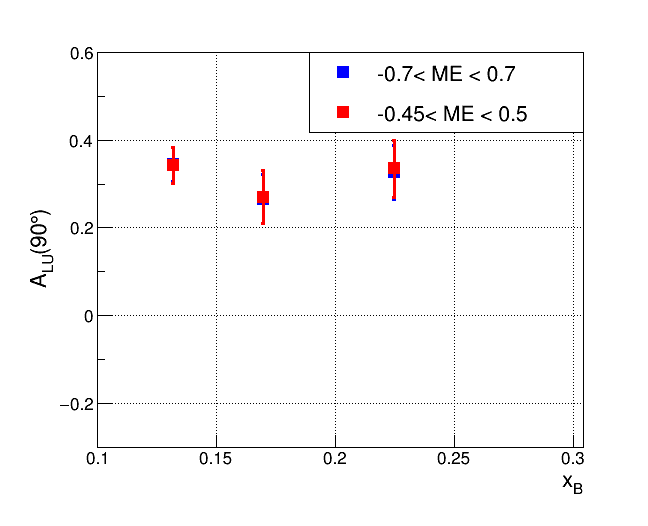
\includegraphics[height=7.5cm]{fig_new/A_LU_He_90_vs_xB.png}
       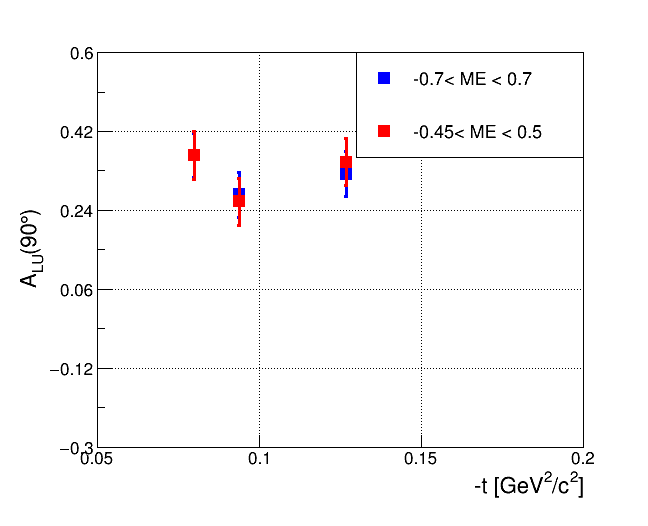
\includegraphics[height=7.5cm]{fig_new/A_LU_He_90_vs_t.png}
       \caption{The extracted asymmetry at $\phi = 90 ^{\circ}$ from
          fitting the asymmetries in fig \ref{fig:BSA_ME_bins_sig} as a 
       function of $Q^{2}$, $x_{B}$ and $-t$ with cutting the tails in red and 
    without cutting the tails in blue.  }
   \label{fig:ALU_ME_bins_sig}
    \end{figure}




\end{enumerate}

\item \textcolor{blue}{Regarding the listed bin by bin systematic errors, they 
   were extracted from the variation of the reconstructed asymmetries such as 
in figures 4.23 and 4.29 in the analysis note. The end of section 4.7 has been 
modified to include the following details on our error bar calculation:}

In addition to evaluating the systematic uncertainties on $A_{LU}$ at $\phi = 
90^{\circ}$, we performed bin by bin, in $\phi$, extraction of these 
uncertainties. For instance, regarding the bin extraction from the source 'data 
binning' listed in table 4.2, the uncertainty is calculated as the difference 
between the two reconstructed asymmetries.  Similar procedures have been 
carried out for the other studies, and finally all the contributions were added 
quadratically. These systematic uncertainties will be shown with the final 
asymmetry results in the following chapter.

\end{enumerate}

